\chapter{TÍNH TOÁN, THIẾT KẾ HỆ THỐNG ĐIỆN}
    \section{Thiết kế sơ đồ nguyên lý điện}
        \begin{figure}[H]
            \centering
            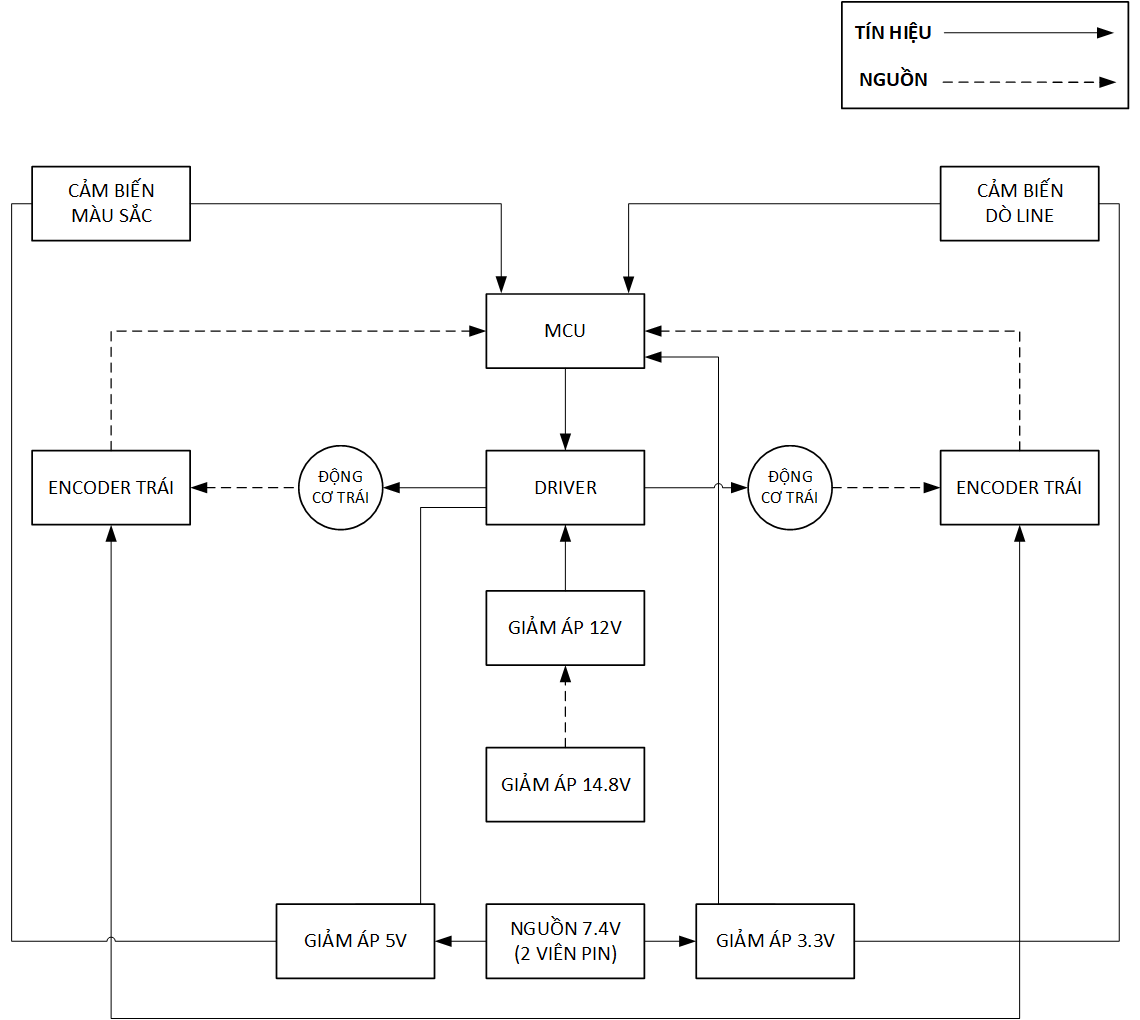
\includegraphics[width=1\textwidth]{pictures/chapter4/c4_p1_ElectricalFlow.png}
            \caption{Sơ đồ nguyên lý điện của hệ thống}
            \label{fig:4-1}
        \end{figure}
    \section{Thiết kế mạch cảm biến}
        \hspace*{0.6cm}Theo tài liệu tham khảo \cite{vishay_tcrt5000_1}, ta có bảng đặc tính kỹ thuật của cảm biến TCRT5000 như sau:
        \begin{table}[H]
            \centering
            \caption{Đặc tính kỹ thuật của cảm biến TCRT5000}
            \label{tab:4-1}
            \begin{tabular}{|c|c|}
                \hline
                \textbf{Thông số} & \textbf{Giá trị} \\
                \hline
                Khoảng cách hoạt động & 0.2 - 15 (mm) \\
                \hline
                Kích thước bao & 10.2 x 5.8 x 7 (mm) \\
                \hline
                Góc phát & $16^{\circ}$ \\
                \hline
                Góc thu & $30^{\circ}$ \\
                \hline
                $I_{C}$ (max) & 100 (mA) \\
                \hline
                $I_{F}$ (max) & 60 (mA) \\
                \hline
            \end{tabular}
        \end{table}
        \subsection{Tính chọn điện trở cho cảm biến dò line}
            \begin{figure}[H]
                \centering
                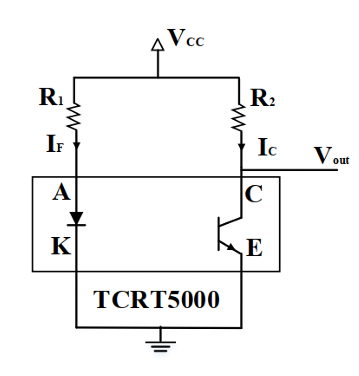
\includegraphics[width=0.3\textwidth]{pictures/chapter4/c4_p2_TCRT5000Schematic.png}
                \caption{Sơ đồ mạch điện TCRT5000}
                \label{fig:4-4}
            \end{figure}
            \hspace*{0.6cm}Dựa vào đường đặc tuyến trên datasheet, ta chọn $V_{F} = 1.1$ (V) và $I_{F} = 10$ (mA).\\
            \begin{figure}[H]
                \centering
                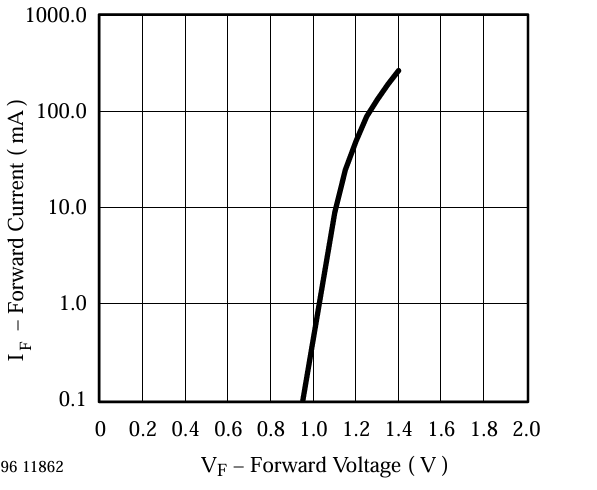
\includegraphics[width=0.5\textwidth]{pictures/chapter4/c4_p3_Voltage&Current.png}
                \caption{Đường đặc tuyến $V_{F}$ và $I_{F}$ của TCRT5000}
                \label{fig:4-5}
            \end{figure}
            Để tính điện trở R1, ta sử dụng công thức:
            \begin{equation}
                R_{1} = \frac{V_{CC} - V_{F}}{I_{F}} = \frac{3.3 - 1.1}{0.01} = 220 \Omega
                \label{eq:4-1}
            \end{equation}
            \hspace*{0.6cm}Chọn điện trở R1 là $220 \Omega$ theo tiêu chuẩn trên thị trường.\\[0.4cm]
            \hspace*{0.6cm}Từ đường đặc tuyến $I_{C} - I_{F}$. Với $I_{F} = 10$ (mA) $\Rightarrow$ $I_{C} \approx 1$ (mA).
            \begin{figure}[H]
                \centering
                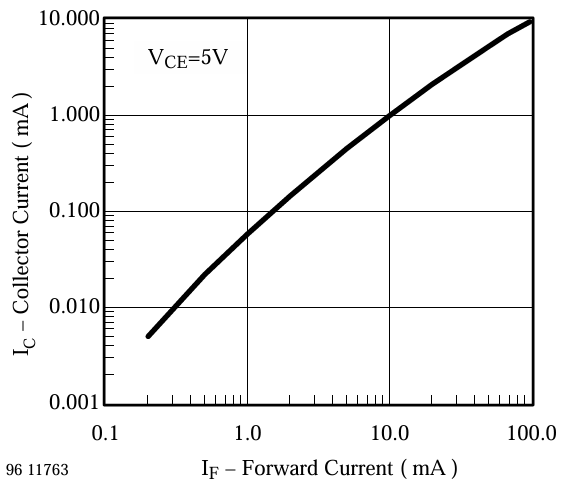
\includegraphics[width=0.5\textwidth]{pictures/chapter4/c4_p4_IC&IF.png}
                \caption{Đường đặc tuyến $I_{C}$ và $I_{F}$ của TCRT5000}
                \label{fig:4-6}
            \end{figure}
            Từ đường đặc tuyến $V_{CE} - I_{C} - I_{F}$, với $I_{C} = 1$ (mA) và $I_{F} = 10$ (mA) $\Rightarrow$ $V_{CE} \approx 1$ (V).\\
            \begin{figure}[H]
                \centering
                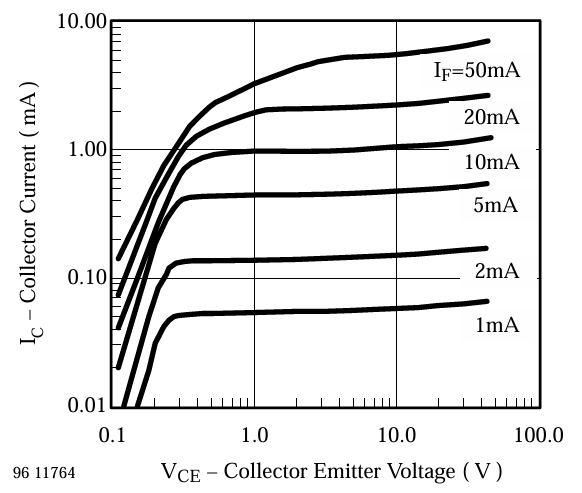
\includegraphics[width=0.5\textwidth]{pictures/chapter4/c4_p5_VCE&IC&IF.png}
                \caption{Đường đặc tuyến $V_{CE}$, $I_{C}$ và $I_{F}$ của TCRT5000}
                \label{fig:4-7}
            \end{figure}
            Từ đó, ta tính điện trở R2:
            \begin{equation}
                R_{2} = \frac{V_{CC} - V_{CE}}{I_{C}} = \frac{3.3 - 1}{0.001} = 2300 \Omega
                \label{eq:4-2}
            \end{equation}
            \hspace*{0.6cm}Chọn điện trở R2 là $2.4 k\Omega$ theo tiêu chuẩn trên thị trường.
        \subsection{Xác định cách đặt cảm biến}
            \hspace*{0.6cm}Có 2 cách đặt cảm biến dò line:
            \begin{itemize}
                \item Trục giữa của bộ phát (S) và thu (E) vuông góc với biên phân cách sáng – tối (Position 1).
                \item Trục giữa của bộ phát (S) và thu (E) song song với biên phân cách sáng – tối (Position 2).
            \end{itemize}
            \begin{figure}[H]
                \centering
                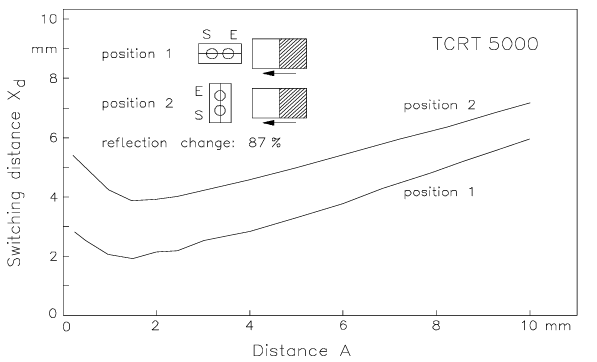
\includegraphics[width=0.8\textwidth]{pictures/chapter4/c4_p6_SensorPosition.png}
                \caption{So sánh độ phân giải của cảm biến khi đặt ở 2 vị trí khác nhau}
                \label{fig:4-8}
            \end{figure}
            \hspace*{0.6cm}Từ hình trên, ta thấy vị trí đặt cảm biến như Position 1 sẽ cho độ phân giải cao hơn so với Position 2. Do đó, ta chọn cách đặt cảm biến ở Position 1.
        \subsection{Xác định khoảng cách giữa cảm biến dò line và sa bàn}
            \hspace*{0.6cm}Theo datasheet, trong khoảng cách từ 0.2 - 15 mm thì cảm biến cho kết quả tốt nhất. Do đó tiến hành đo giá trị ADC từ cảm biến trong khoảng 1 - 15mm trên sa bản và thu được kết quả.
            \begin{table}[H]
                \centering
                \caption{Giá trị ADC từ cảm biến dò line ở các khoảng cách khác nhau}
                \label{tab:4-2}
                \begin{tabular}{|c|c|c|c|}
                    \hline
                    \textbf{h (mm)} & \textbf{Giá trị vùng trắng} & \textbf{Giá trị vùng đen} & \textbf{Chênh lệch} \\
                    \hline
                    1 & 39 & 814 & 775 \\
                    \hline
                    2 & 37 & 798 & 761 \\
                    \hline
                    3 & 37 & 785 & 748 \\
                    \hline
                    4 & 34 & 786 & 752 \\
                    \hline
                    5 & 36 & 793 & 757 \\
                    \hline
                    6 & 37 & 797 & 760 \\
                    \hline
                    7 & 36 & 804 & 768 \\
                    \hline
                    \rowcolor{yellow!50}
                    8 & 38 & 841 & 803 \\
                    \hline
                    \rowcolor{yellow!50}
                    9 & 39 & 856 & 817 \\
                    \hline
                    \rowcolor{yellow!50}
                    10 & 40 & 864 & 824 \\
                    \hline
                    \rowcolor{yellow!50}
                    11 & 41 & 878 & 837 \\
                    \hline
                    \rowcolor{yellow!50}
                    12 & 53 & 894 & 841 \\
                    \hline
                    13 & 134 & 872 & 738 \\
                    \hline
                    14 & 162 & 936 & 774 \\
                    \hline
                    15 & 231 & 896 & 665 \\
                    \hline
                \end{tabular}
            \end{table}
            \begin{figure}[H]
                \centering
                \begin{tikzpicture}
                    \begin{axis}[
                        width=14cm,
                        height=8cm,
                        xlabel={Khoảng cách h (mm)},
                        ylabel={Giá trị ADC},
                        legend pos=north west,
                        grid=major,
                        xmin=0, xmax=16,
                        ymin=0, ymax=1000,
                        mark size=2pt
                    ]
                    
                    % Đường giá trị vùng trắng
                    \addplot[color=blue, mark=o, thick] coordinates {
                        (1,39) (2,37) (3,37) (4,34) (5,36) (6,37) (7,36) 
                        (8,38) (9,39) (10,40) (11,41) (12,53) (13,134) 
                        (14,162) (15,231)
                    };
                    \addlegendentry{Vùng trắng}
                    
                    % Đường giá trị vùng đen
                    \addplot[color=red, mark=square, thick] coordinates {
                        (1,814) (2,798) (3,785) (4,786) (5,793) (6,797) (7,804) 
                        (8,841) (9,856) (10,864) (11,878) (12,894) (13,872) 
                        (14,936) (15,896)
                    };
                    \addlegendentry{Vùng đen}
                    
                    % Highlight vùng tối ưu (8-12mm)
                    \addplot[color=gray, fill=yellow, fill opacity=0.3, draw=none] 
                    coordinates {(8,0) (8,1000) (12,1000) (12,0)} \closedcycle;
                    
                    \end{axis}
                \end{tikzpicture}
                \caption{Đồ thị giá trị ADC theo khoảng cách cảm biến}
                \label{fig:4.9}
            \end{figure}

            % Vẽ đồ thị chênh lệch
            \begin{figure}[H]
                \centering
                \begin{tikzpicture}
                    \begin{axis}[
                        width=14cm,
                        height=8cm,
                        xlabel={Khoảng cách h (mm)},
                        ylabel={Chênh lệch giá trị ADC},
                        grid=major,
                        xmin=0, xmax=16,
                        ymin=600, ymax=900,
                        mark size=2pt
                    ]
                    
                    % Đường chênh lệch
                    \addplot[color=green, mark=triangle, thick] coordinates {
                        (1,775) (2,761) (3,748) (4,752) (5,757) (6,760) (7,768) 
                        (8,803) (9,817) (10,824) (11,837) (12,841) (13,738) 
                        (14,774) (15,665)
                    };
                    
                    % Highlight vùng tối ưu
                    \addplot[color=gray, fill=green, fill opacity=0.2, draw=none] 
                    coordinates {(8,600) (8,900) (12,900) (12,600)} \closedcycle;
                    
                    \end{axis}
                \end{tikzpicture}
                \caption{Đồ thị chênh lệch giá trị ADC theo khoảng cách}
                \label{fig:4.10}
            \end{figure}
            Từ bảng trên ta thấy trong khoảng h từ 8 - 12 mm thì chênh lệch giá trị ADC giữa vùng trắng và vùng đen là lớn nhất và ổn định nhất. Do đó, ta tiếp tục cho cảm biến đi ngang qua đường line với quãng đường 20mm quanh ranh giới trắng và đen trong khoảng h từ 8 - 12 mm để xác định độ cao thích hợp nhất.
            \begin{table}[H]
                \centering
                \caption{Giá trị ADC khi cảm biến đi qua đường line với khoảng cách khác nhau}
                \label{tab:4-3}
                \begin{tabular}{|c|c|c|c|c|c|c|c|c|c|c|c|}
                    \hline
                    \textbf{h} & \textbf{0} & \textbf{1} & \textbf{2} & \textbf{3} & \textbf{4} & \textbf{5} & \textbf{6} & \textbf{7} & \textbf{8} & \textbf{9} & \textbf{10} \\
                    \hline
                    \textbf{8} & 45 & 44 & 54 & 135 & 200 & 285 & 345 & 491 & 623 & 655 & 713 \\
                    \hline
                    \textbf{9} & 43 & 43 & 52 & 130 & 190 & 280 & 340 & 503 & 625 & 662 & 721 \\
                    \hline
                    \textbf{10} & 45 & 43 & 52 & 93 & 195 & 277 & 332 & 505 & 609 & 674 & 739 \\
                    \hline
                    \textbf{11} & 43 & 43 & 50 & 112 & 189 & 263 & 349 & 482 & 615 & 663 & 698 \\
                    \hline
                    \textbf{12} & 41 & 40 & 44 & 90 & 167 & 233 & 313 & 473 & 591 & 639 & 679 \\
                    \hline
                \end{tabular}
                \begin{tabular}{|c|c|c|c|c|c|c|c|c|c|c|}
                    \hline
                    \textbf{h} & \textbf{11} & \textbf{12} & \textbf{13} & \textbf{14} & \textbf{15} & \textbf{16} & \textbf{17} & \textbf{18} & \textbf{19} & \textbf{20} \\
                    \hline
                    \textbf{8} & 790 & 819 & 850 & 855 & 865 & 870 & 855 & 878 & 875 & 877 \\
                    \hline
                    \textbf{9} & 785 & 823 & 845 & 850 & 860 & 865 & 850 & 873 & 870 & 872 \\
                    \hline
                    \textbf{10} & 794 & 836 & 848 & 853 & 863 & 863 & 862 & 862 & 860 & 863 \\
                    \hline
                    \textbf{11} & 787 & 825 & 857 & 861 & 867 & 873 & 877 & 877 & 875 & 876 \\
                    \hline
                    \textbf{12} & 765 & 803 & 825 & 836 & 844 & 849 & 849 & 852 & 857 & 855 \\
                    \hline
                \end{tabular}
            \end{table}

            \begin{figure}[H]
                \centering
                \begin{tikzpicture}
                    \begin{axis}[
                        width=16cm,
                        height=10cm,
                        xlabel={Vị trí cảm biến (mm)},
                        ylabel={Giá trị ADC},
                        legend pos=north west,
                        grid=major,
                        xmin=-1, xmax=21,
                        ymin=0, ymax=1000,
                        mark size=1.5pt,
                        legend style={font=\small}
                    ]
                    
                    % h = 8mm (màu xanh dương)
                    \addplot[color=blue, mark=none, thick, smooth] coordinates {
                        (0,45) (1,44) (2,54) (3,135) (4,200) (5,285) (6,345) (7,491) (8,623) (9,655) 
                        (10,713) (11,790) (12,819) (13,850) (14,855) (15,865) (16,870) (17,855) (18,878) (19,875) (20,877)
                    };
                    \addlegendentry{8}
                    
                    % h = 9mm (màu cam)
                    \addplot[color=orange, mark=none, thick, smooth] coordinates {
                        (0,43) (1,43) (2,52) (3,130) (4,190) (5,280) (6,340) (7,503) (8,625) (9,662) 
                        (10,721) (11,785) (12,823) (13,845) (14,850) (15,860) (16,865) (17,850) (18,873) (19,870) (20,872)
                    };
                    \addlegendentry{9}
                    
                    % h = 10mm (màu đỏ - highlight)
                    \addplot[color=red, mark=none, thick, smooth] coordinates {
                        (0,45) (1,43) (2,52) (3,93) (4,195) (5,277) (6,332) (7,505) (8,609) (9,674) 
                        (10,739) (11,794) (12,836) (13,848) (14,853) (15,863) (16,863) (17,862) (18,862) (19,860) (20,863)
                    };
                    \addlegendentry{10}
                    
                    % h = 11mm (màu vàng)
                    \addplot[color=yellow!80!black, mark=none, thick, smooth] coordinates {
                        (0,43) (1,43) (2,50) (3,112) (4,189) (5,263) (6,349) (7,482) (8,615) (9,663) 
                        (10,698) (11,787) (12,825) (13,857) (14,861) (15,867) (16,873) (17,877) (18,877) (19,875) (20,876)
                    };
                    \addlegendentry{11}
                    
                    % h = 12mm (màu xanh nhạt)
                    \addplot[color=cyan, mark=none, thick, smooth] coordinates {
                        (0,41) (1,40) (2,44) (3,79) (4,167) (5,233) (6,313) (7,473) (8,591) (9,639) 
                        (10,679) (11,765) (12,803) (13,825) (14,836) (15,844) (16,849) (17,849) (18,852) (19,857) (20,855)
                    };
                    \addlegendentry{12}
                    
                    % Đánh dấu vị trí chuyển line tại x = 10
                    \addplot[color=black, mark=none, thick, dashed] coordinates {(10,0) (10,1000)};
                    
                    % Thêm text đánh dấu
                    \node[anchor=south] at (axis cs:10,900) {\textbf{Chuyển line}};
                    \node[anchor=south] at (axis cs:10,850) {\textbf{(Vị trí 10)}};
                    
                    % Đánh dấu vùng trước và sau line
                    \node[anchor=center] at (axis cs:5,600) {\textbf{Vùng trắng}};
                    \node[anchor=center] at (axis cs:15,600) {\textbf{Vùng đen}};
                    
                    \end{axis}
                \end{tikzpicture}
                \caption{Biểu đồ giá trị ADC khi cảm biến đi qua đường line}
                \label{fig:4-11}
            \end{figure}
            Từ bảng và đồ thị trên, ta thấy tại h = 10mm, cảm biến cho kết quả chuyển tiếp rõ ràng và nhanh nhất giữa nền trắng và nền đen. Do đó, ta chọn khoảng cách từ cảm biến dò line đến sa bàn là 10mm.

        \subsection{Xác định khoảng cách giữa các cảm biến}
            \begin{figure}[H]
                \centering
                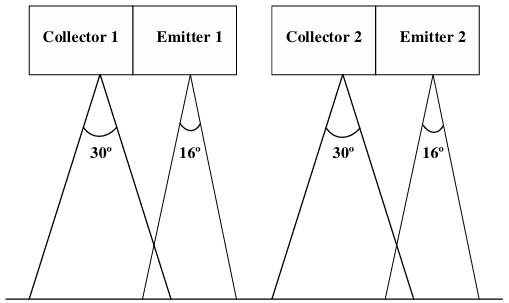
\includegraphics[width=0.7\textwidth]{pictures/chapter4/c4_p7_DistanceCollectorEmitter1.png}
                \label{fig:4-12}
                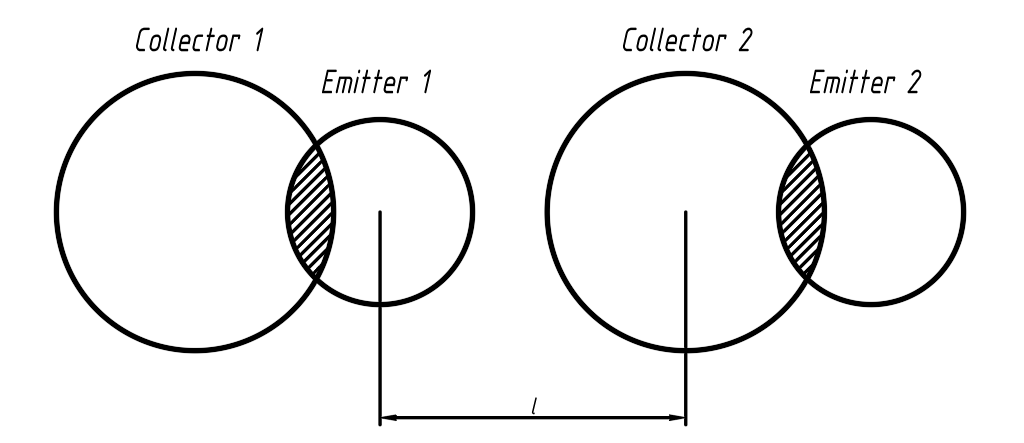
\includegraphics[width=0.8\textwidth]{pictures/chapter4/c4_p8_DistanceCollectorEmitter2.png}
                \caption{Khoảng cách giữa các vùng thu và vùng phát}
                \label{fig:4-13}
                \end{figure}
            \hspace*{0.6cm}Với h = 10mm, ta tính khoảng cách giữa vùng phát và vùng thu liền kề nhau tối thiểu để không bị giao thoa là:
            \begin{align}
                l_{min} &= (r + R) \label{eq:4-3} \\
                        &= (h +0.7) \times \tan{8^{\circ}} + (h + 0.7) \times \tan{15^{\circ}} \nonumber \\
                        &= (10 + 0.7) \times \tan{8^{\circ}} + (10 + 0.7) \times \tan{15^{\circ}} \nonumber \\
                        &= 4.4 \text{ (mm)} \nonumber
            \end{align}
            \hspace*{0.6cm}Khoảng cách tối thiểu giữa 2 cảm biến là:
            \begin{align}
                d_{min} = l_{min} + d = 4.4 + 3.8 = 8.2 \text{ (mm)}
                \label{eq:4-4}
            \end{align}
            \hspace*{0.6cm}Dựa vào datasheet, ta có chiều dài của cảm biến TCRT5000 là 10.2 mm (bố trí nằm ngang). Do đó, với độ cao $h = 10$ mm thì chắc chắn hai cảm biến liền kề không ảnh hưởng nhau.\\[0.4cm]
            \begin{figure}[H]
                \centering
                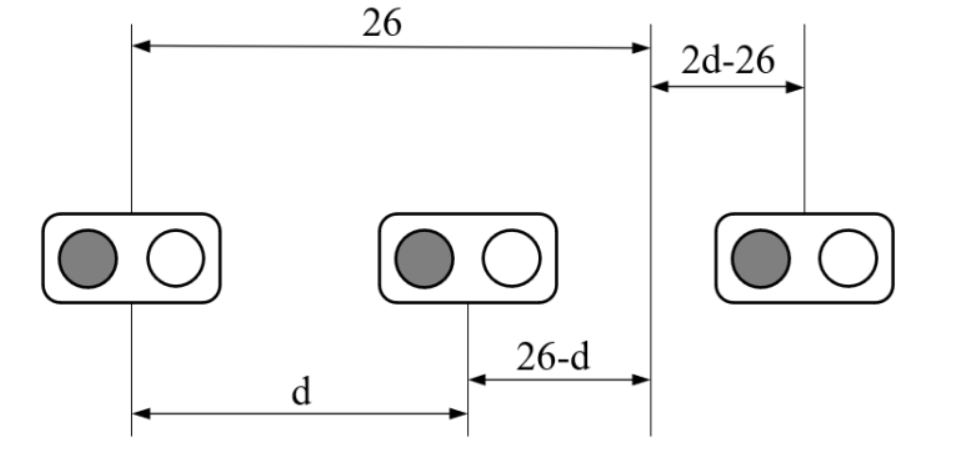
\includegraphics[width=0.8\textwidth]{pictures/chapter4/c4_p9_SensorDistance.png}
                \caption{Khoảng cách giữa các cảm biến dò line}
                \label{fig:4-14}
            \end{figure}
            Do line có bề rộng là 26mm nên tối đa có 3 cảm biến có vùng phát hiện nằm trong line. Bên cạnh đó, khi hoạt động sẽ có trường hợp cảm biến rơi vào vùng bất định thì giá trị analog trả về từ cảm biến sẽ như nhau. Do đó, không thể tính toán sai số để xác định được vị trí cảm biến so với đường tâm line. \\
            \hspace*{0.6cm}Ta xét các trường hợp:
            \begin{itemize}
                \item Trường hợp 1: Khi di chuyển sang phải trong khoảng 26 - d thì có 2 led nằm trong line nên thuđược giá trị analog là như nhau dẫn đến cảm biến rơi vào vùng bất định. 
                \item Trường hợp 2: Khi di chuyển sang trái trong khoảng 2d - 26 thì chỉ có 1 led nằm trên đường line và cũng rơi vào vùng bất định. 
            \end{itemize}
            \hspace*{0.6cm}Do đó để hạn chế việc cảm biến rơi vào vùng bất định thì lựa chọn khoảng cách $d$ sao cho $f_1 = 26 - d$ và $f_2 = 2d - 26$ là nhỏ nhất. \\
            \hspace*{0.6cm}Do $f_1$ là hàm đơn điệu giảm, $f_2$ là hàm đơn điệu tăng nên để $f_1$ và $f_2$ là nhỏ nhất thì ta chọn $f_1 = f_2$. Từ đó ta có:
            \begin{align}
                f_1 &= f_2 \label{eq:4-5}\\
                \Rightarrow 26 - d &= 2d - 26 \nonumber \\
                \Rightarrow d &= 17.33 \text{ (mm)} \nonumber
            \end{align}
        \subsection{Thiết kế sơ đồ nguyên lý mạch cảm biến}
            \hspace*{0.6cm}Dựa vào các tính toán trên, ta thiết kế sơ đồ nguyên lý mạch cảm biến như sau:
            \begin{itemize}
                \item Sử dụng 5 cảm biến TCRT5000 được bố trí nằm ngang vuông góc theo đường line.
                \item Khoảng cách từ cảm biến đến sa bàn là 10mm.
                \item Khoảng cách giữa các cảm biến là 17mm.
                \item Điện trở R1 là 220$\Omega$ và R2 là 2.4k$\Omega$.
            \end{itemize}
            \begin{figure}[H]
                \centering
                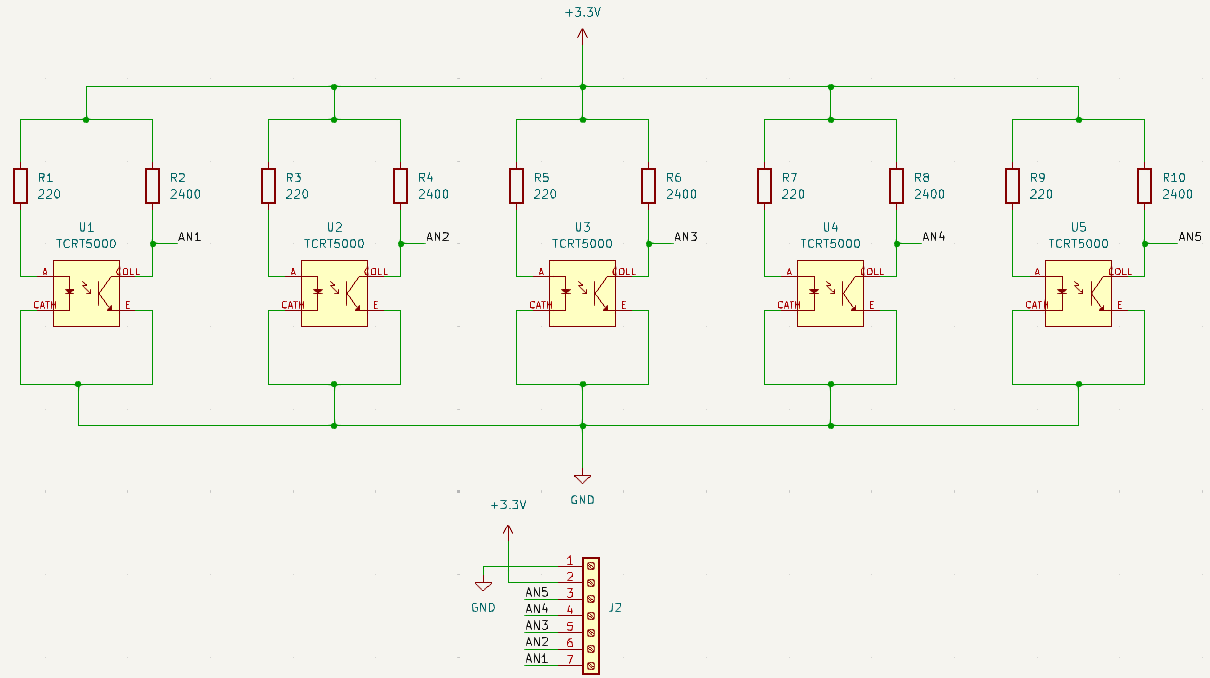
\includegraphics[width=1\textwidth]{pictures/chapter4/c4_p10_SensorSchematic.png}
                \caption{Sơ đồ nguyên lý mạch cảm biến dò line}
                \label{fig:4-15}
            \end{figure}
        \subsection{Thiết kế PCB mạch cảm biến}

            \hspace*{0.6cm}Dựa vào sơ đồ nguyên lý mạch cảm biến, ta tiến hành thiết kế PCB cho mạch cảm biến dò line. Sơ đồ thiết kế PCB được trình bày như hình \ref{fig:4-16}.

            \begin{figure}[H]
                \centering
                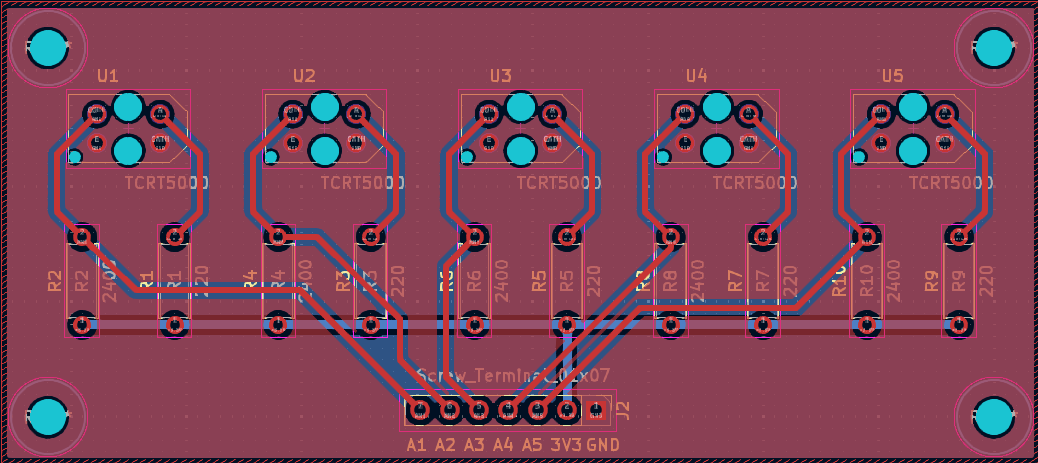
\includegraphics[width=1\textwidth]{pictures/chapter4/c4_p11_SensorPCB.png}
                \caption{Sơ đồ thiết kế PCB mạch cảm biến dò line}
                \label{fig:4-16}
            \end{figure}
        \subsection{Calib và tuyến tính hóa cảm biến}
            \hspace*{0.6cm}Mỗi cảm biến dò line sẽ trả về tín hiệu analog khác nhau trong cùng điều kiện. Do đó, việc calib cảm biến là vô cùng cần thiết. Lựa chọn phương pháp calib bằng công thức:
            \begin{align}
                y_i = y_{min} + \frac{(y_{max} - y_{min})(x_{ij} - x_{min, i})}{x_{max, i} - x_{min, i}} 
                \label{eq:4-6}
            \end{align}
            \hspace*{0.6cm}Trong đó:
            \begin{itemize}
                \item $x_{max,i}$ và $x_{min,i}$: giá trị analog lớn nhất và nhỏ nhất của cảm biến thứ $i$.
                \item $y_{max}$ và $y_{min}$: giá trị analog lớn nhất và nhỏ nhất mà ta mong muốn cho tất cả cảm biến.
                \item $x_{ij}$: giá trị analog đọc về từ cảm biến thứ $i$.
                \item $y_{i0}$: giá trị analog đọc về sau khi đã calib của cảm biến thứ $i$.
            \end{itemize}
            \begin{table}[H]
                \centering
                \caption{Bảng giá trị analog của cảm biến trước khi calib ở độ cao h = 10mm}
                \label{tab:4-4}
                \begin{tabular}{|c|c|c|}
                    \hline
                    \textbf{Cảm biến} & $\mathbf{x_{max,i}}$ & $\mathbf{x_{min,i}}$  \\
                    \hline
                    Cảm biến 1 & 870 & 54  \\
                    \hline
                    Cảm biến 2 & 805 & 51  \\
                    \hline
                    Cảm biến 3 & 872 & 73  \\
                    \hline
                    Cảm biến 4 & 855 & 65  \\
                    \hline
                    Cảm biến 5 & 863 & 88  \\
                    \hline
                \end{tabular}
            \end{table}
            \hspace*{0.6cm}Dựa vào giá trị trung bình, ta có được giá trị mong muốn: $y_{max} = 853$ và $y_{min} = 66$.\\
            \hspace*{0.6cm}Từ đó ta có công thức calib cho từng cảm biến:
            \begin{itemize}
                \item Cảm biến 1:
                \begin{align*}
                    y_1 = 66 + \frac{(853 - 66)(x_{1j} - 54)}{870 - 54} = 66 + 0.88(x_{1j} - 54)
                \end{align*}
                \item Cảm biến 2:
                \begin{align*}
                    y_2 = 66 + \frac{(853 - 66)(x_{2j} - 51)}{805 - 51} = 66 + 0.95(x_{2j} - 51)
                \end{align*}
                \item Cảm biến 3:
                \begin{align*}
                    y_3 = 66 + \frac{(853 - 66)(x_{3j} - 73)}{872 - 73} = 66 + 0.88(x_{3j} - 73)
                \end{align*}
                \item Cảm biến 4:
                \begin{align*}
                    y_4 = 66 + \frac{(853 - 66)(x_{4j} - 65)}{855 - 65} = 66 + 0.91(x_{4j} - 65)
                \end{align*}
                \item Cảm biến 5:
                \begin{align*}
                    y_5 = 66 + \frac{(853 - 66)(x_{5j} - 88)}{863 - 88} = 66 + 0.89(x_{5j} - 88)
                \end{align*}
            \end{itemize}
        \subsection{Tìm giá trị sai số theo phương pháp trung bình trọng số}
            \hspace*{0.6cm}Giá sử tọa độ của 5 cảm biến lần lượt là $x_1, x_2, x_3, x_4, x_5$ so với tâm đường line và các giá trị analog tương ứng là $y_1, y_2, y_3, y_4, y_5$. Từ đó, ta tìm được vị trí xe so với tâm đường line theo công thức sau:
            \begin{equation}
                X = L_{cb} \times \frac{\sum_{i=1}^{5} x_i y_i}{\sum_{i=1}^{5} y_i} = 17 \times \frac{2(y_5 - y_1) + (y_4 - y_2)}{y_1 + y_2 + y_3 + y_4 + y_5}
                \label{eq:4-7}
            \end{equation}

            Tiến hành thực nghiệm đọc tín hiệu cảm biến với bước nhảy 1 mm, giới hạn từ $-30$ mm tới $30$ mm so với tâm đường line bằng máy in 3D theo quy trình sau:
            \begin{itemize}
                \item Bước 1: Tiến hành gá cụm cảm biến lên cụm in của máy in 3D.
                \item Bước 2: Di chuyển trục z về vị trí home là vị trí cách mặt in đúng bằng khoảng cách từ cảm biến đến line theo tính toán (10 mm).
                \item Bước 3: Dịch chỉnh trục x sao cho cụm cảm biến có cảm biến giữa nằm đúng vị trí tâm line là vị trí mà giá trị cảm biến giữa đọc về lớn nhất.
                \item Bước 4: Di chuyển cụm in sang trái 30 mm và sang phải 30 mm để tiến hành đọc giá trị analog của từng cảm biến.
            \end{itemize}
            \begin{figure}[H]
                \centering
                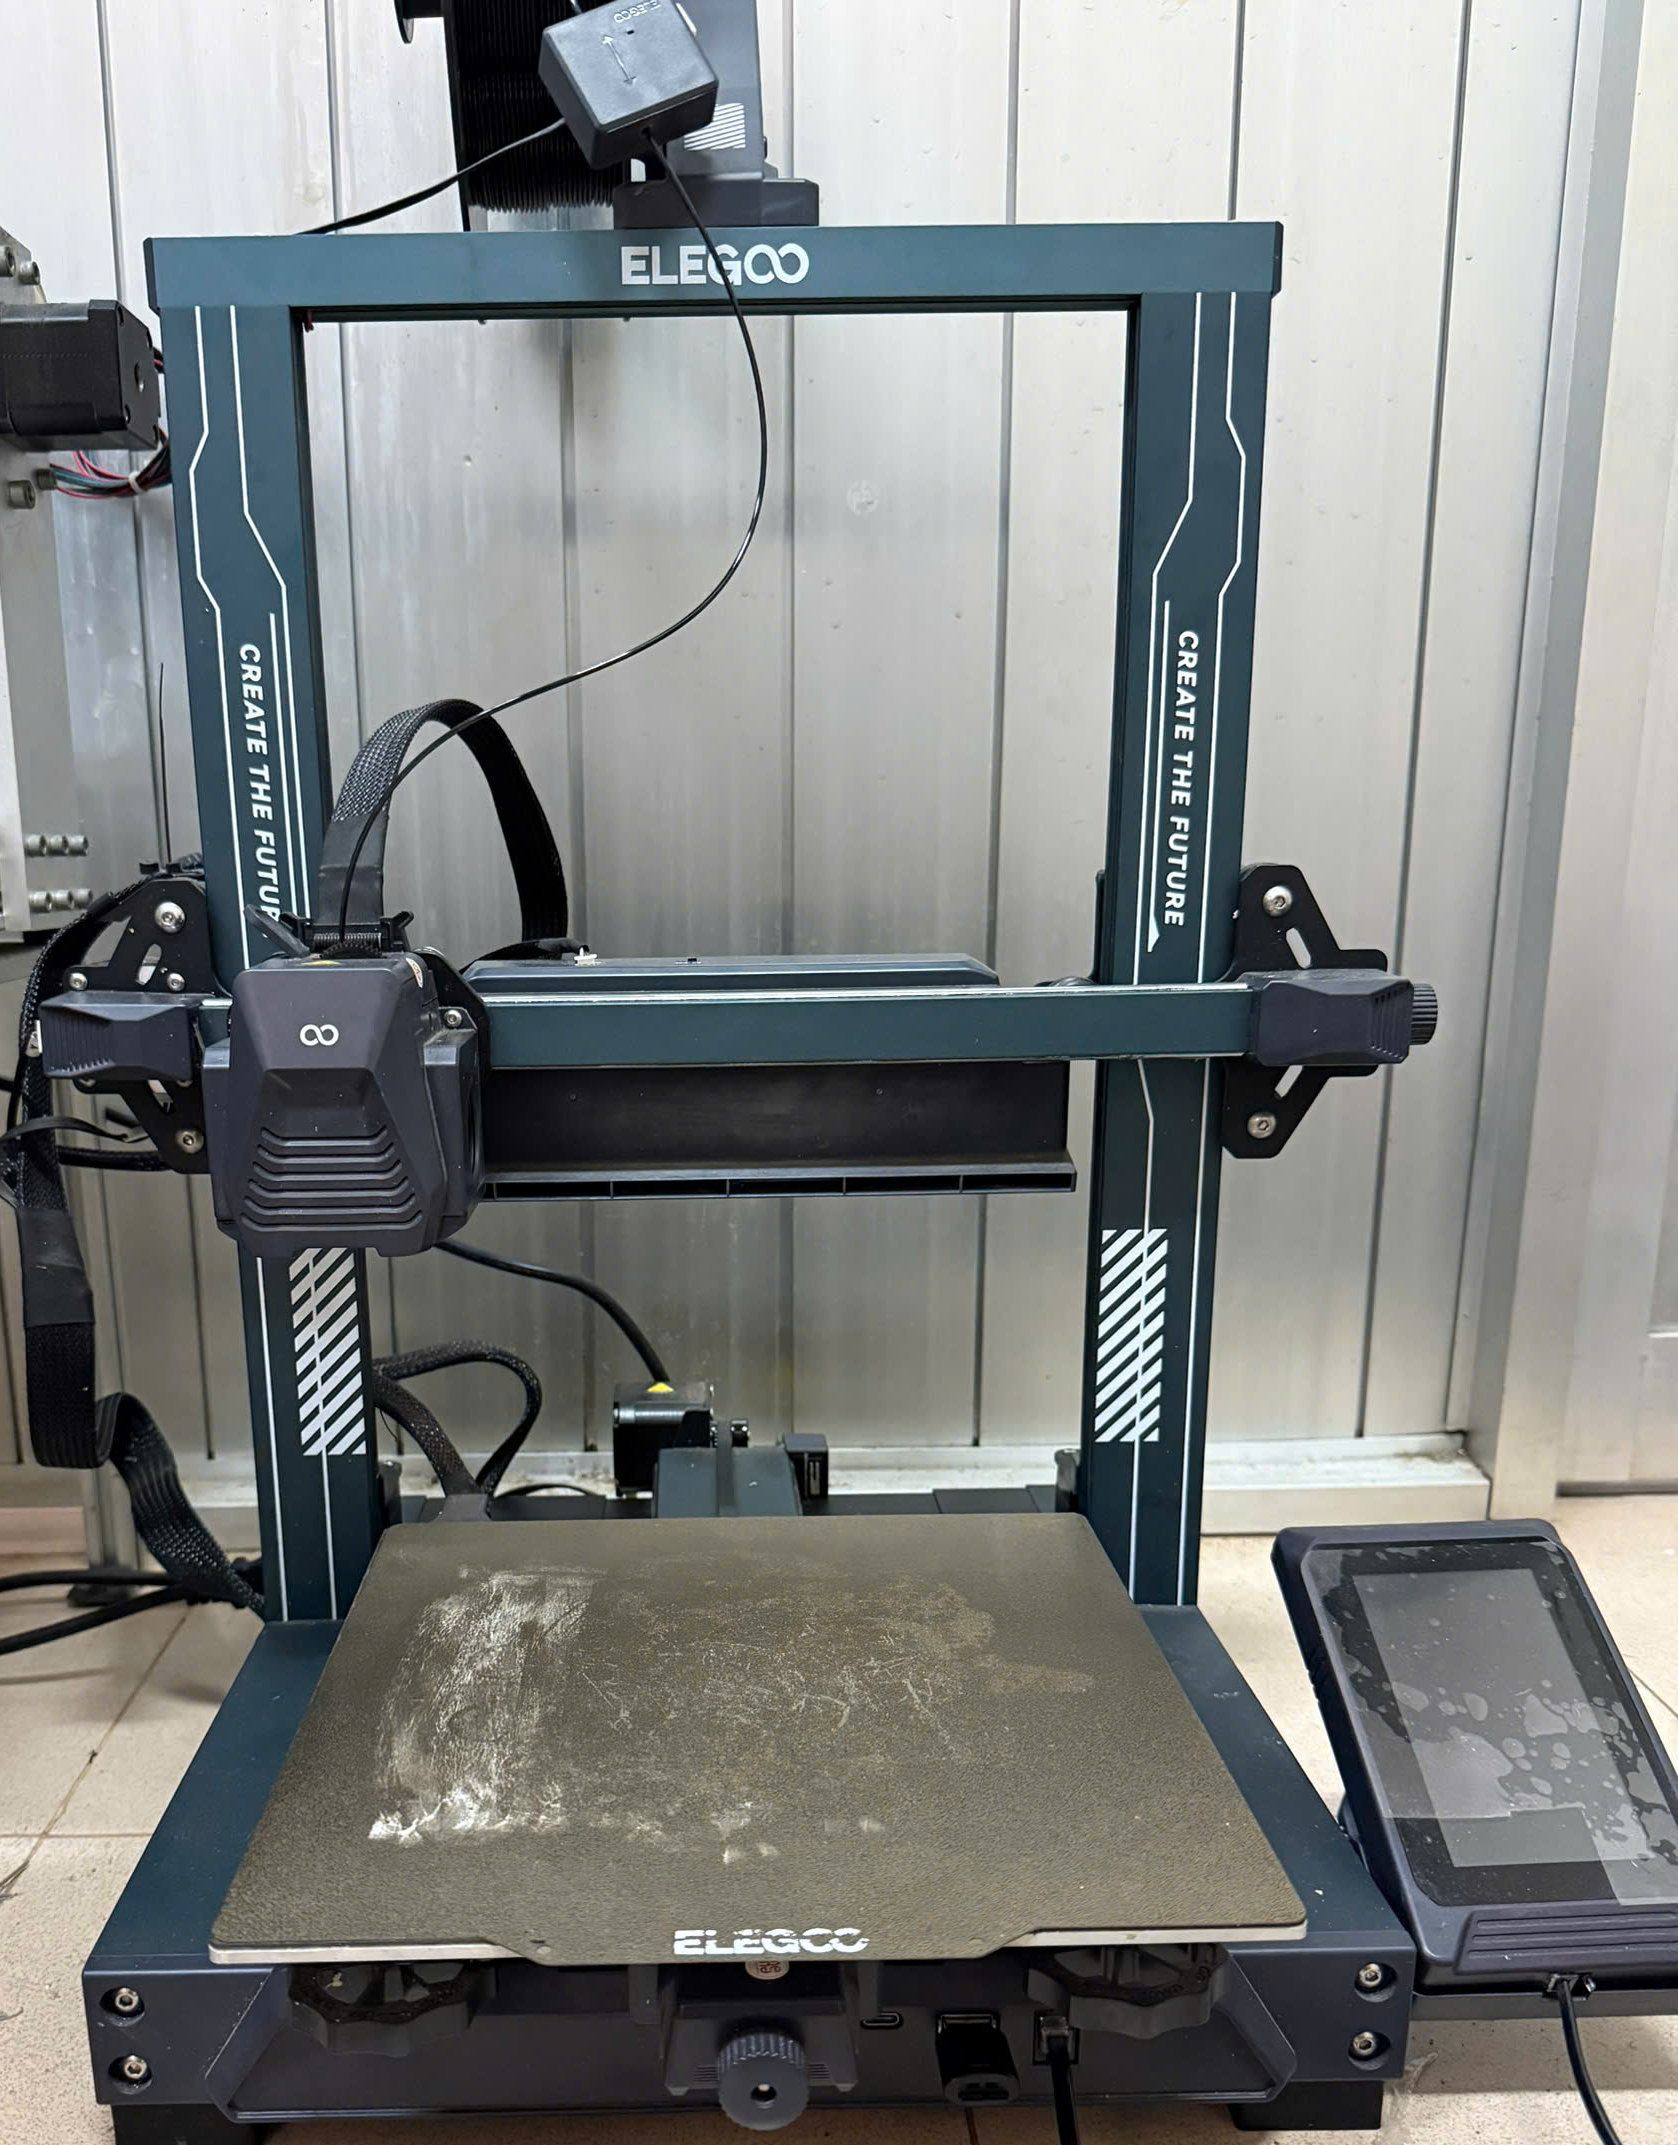
\includegraphics[width=0.6\textwidth]{pictures/chapter4/c4_p16_3DPrinter.png}
                \caption{Máy in 3D dùng để hiệu chuẩn cảm biến dò line}
                \label{fig:4-17}
            \end{figure}
        
            \begin{longtable}{|c|c|c|}
                \caption{Bảng tính toán giá trị sai số giữa vị trí trên thực tế và vị trí tính toán}
                \label{tab:4-5} \\
                \hline
                \textbf{Vị trí (mm)} & \textbf{Giá trị tính toán (mm)} & \textbf{Sai số (mm)} \\
                \hline
                \endfirsthead
                
                \hline
                \textbf{Vị trí (mm)}  & \textbf{Giá trị tính toán (mm)} & \textbf{Sai số (mm)} \\
                \hline
                \endhead
                0 & 0.271428571 & -0.271428571 \\
                \hline
                1 & 0.495008319 & 0.504991681 \\
                \hline
                2 & 2.248142645 & -0.248142645 \\
                \hline
                3 & 4.205958549 & -1.205958549 \\
                \hline
                4 & 5.70234688 & -1.70234688 \\
                \hline
                5 & 6.675065617 & -1.675065617 \\
                \hline
                6 & 7.134005038 & -1.134005038 \\
                \hline
                7 & 7.347029703 & -0.347029703 \\
                \hline
                8 & 7.440652819 & 0.559347181 \\
                \hline
                9 & 7.506713078 & 1.493286922 \\
                \hline
                10 & 7.686354379 & 2.313645621 \\
                \hline
                11 & 8.204347826 & 2.795652174 \\
                \hline
                12 & 9.220866382 & 2.779133618 \\
                \hline
                13 & 10.71843972 & 2.28156028 \\
                \hline
                14 & 12.5566584 & 1.4433416 \\
                \hline
                15 & 12.94961571 & 2.05038429 \\
                \hline
                16 & 13.04991394 & 2.95008606 \\
                \hline
                17 & 13.21570319 & 3.78429681 \\
                \hline
                18 & 14.01160862 & 3.98839138 \\
                \hline
                19 & 16.23355506 & 2.76644494 \\
                \hline
                20 & 18.4286645 & 1.5713355 \\
                \hline
                21 & 20.32566168 & 0.67433832 \\
                \hline
                22 & 21.45665962 & 0.54334038 \\
                \hline
                23 & 22.02743902 & 0.97256098 \\
                \hline
                24 & 22.18875502 & 1.81124498 \\
                \hline
                25 & 22.2288008 & 2.7711992 \\
                \hline
                26 & 22.25314545 & 3.74685455 \\
                \hline
                27 & 22.29408767 & 4.70591233 \\
                \hline
                28 & 22.59401709 & 5.40598291 \\
                \hline
                29 & 23.23741007 & 5.76258993 \\
                \hline
                30 & 24.31478873 & 5.68521127 \\
                \hline
                -30 & -22.63765643 & -7.36234357 \\
                \hline
                -29 & -22.14532148 & -6.85467852 \\
                \hline
                -28 & -21.89844922 & -6.10155078 \\
                \hline
                -27 & -21.79960513 & -5.20039487 \\
                \hline
                -26 & -21.70588235 & -4.29411765 \\
                \hline
                -25 & -21.54179104 & -3.45820896 \\
                \hline
                -24 & -21.11036961 & -2.88963039 \\
                \hline
                -23 & -20.09944751 & -2.90055249 \\
                \hline
                -22 & -18.35491905 & -3.64508095 \\
                \hline
                -21 & -15.75849602 & -5.24150398 \\
                \hline
                -20 & -12.98336106 & -7.01663894 \\
                \hline
                -19 & -12.43197279 & -6.56802721 \\
                \hline
                -18 & -12.26729291 & -5.73270709 \\
                \hline
                -17 & -11.77140482 & -5.22859518 \\
                \hline
                -16 & -10.55522388 & -5.44477612 \\
                \hline
                -15 & -9.357284113 & -5.642715887 \\
                \hline
                -14 & -8.419335706 & -5.580664294 \\
                \hline
                -13 & -7.701092896 & -5.298907104 \\
                \hline
                -12 & -7.182608696 & -4.817391304 \\
                \hline
                -11 & -6.949152542 & -4.050847458 \\
                \hline
                -10 & -6.865708622 & -3.134291378 \\
                \hline
                -9 & -6.833746898 & -2.166253102 \\
                \hline
                -8 & -6.766169154 & -1.233830846 \\
                \hline
                -7 & -6.607287449 & -0.392712551 \\
                \hline
                -6 & -5.884615385 & -0.115384615 \\
                \hline
                -5 & -4.360049322 & -0.639950678 \\
                \hline
                -4 & -1.420972644 & -2.579027356 \\
                \hline
                -3 & 0.014119601 & 3.014119601 \\
                \hline
                -2 & 0.127926421 & 2.127926421 \\
                \hline
                -1 & 0.171428571 & 1.171428571 \\
                \hline        
            \end{longtable}
            \hspace*{0.6cm}Dựa vào số liệu trên, ta thực hiện xấp xỉ tuyến tính giá trị tính toán theo vị trí, thu được phương trình tính xấp xỉ vị trí:
            \begin{align}
                y = 0.8136x - 1.0349
                \label{eq:4-8}
            \end{align}
            Trong đó:
            \begin{itemize}
                \item $y$: giá trị trung bình trọng số (mm).
                \item $x$: vị trí tính toán (mm).
            \end{itemize}
            \begin{figure}[H]
                \centering
                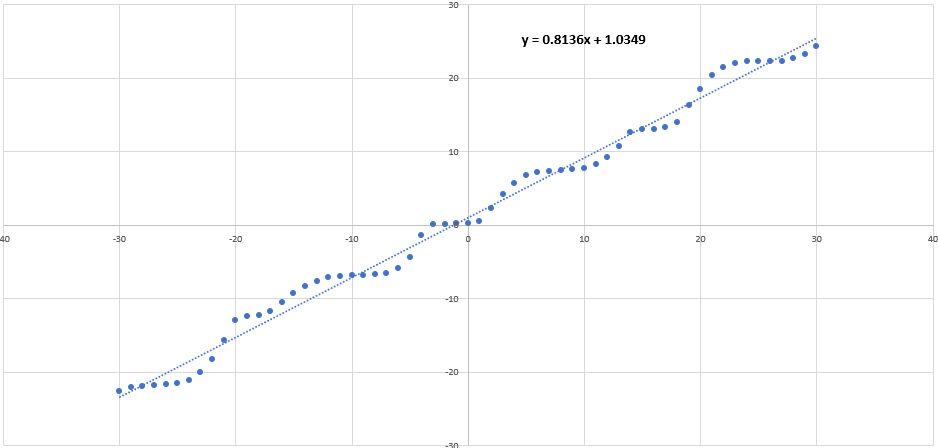
\includegraphics[width=1\textwidth]{pictures/chapter4/c4_p12_LinearRegression.png}
                \caption{Biểu đồ xấp xỉ tuyến tính giá trị tính toán theo vị trí}
                \label{fig:4-8}
            \end{figure}
            \hspace*{0.6cm}Từ bảng số liệu trên, ta có sai số cảm biến lớn nhất đo được là: $e_{max} = 5.8$ mm. \\
    \section{Thiết kế mạch điều khiển} 
        \subsection{Thiết kế mạch nguồn}
            \subsubsection{Nguồn điều khiển}
                \begin{itemize}
                    \item Nguồn điều khiển cần cung cấp cho:
                    \begin{itemize}
                        \item Vi điều khiển STM32F103C8T6: 3.3V
                        \item Mạch cảm biến dò line: 3.3V
                        \item Driver TB6612FNG: 5V
                        \item Cảm biến màu sắc TCS347254: 3.3V
                        \item 2 Encoder: 3.3V
                    \end{itemize}
                    \item Công suất mạch cảm biến:
                    \begin{itemize}
                        \item Công suất tiêu thụ của 5 điện trở $R = 220 \Omega$ trong mạch. \\
                        \begin{align}
                            P_{R1} = 5 \times I_{F}^2 \times R_1 = 5 \times (10.10^{-3})^2 \times 220 = 110 \text{ (mW)}
                        \end{align}
                        \item Công suất tiêu thụ của 5 điện trở $R = 2.4 k\Omega$ trong mạch. \\
                        \begin{align}
                            P_{R2} = 5 \times I_{C}^2 \times R_2 = 5 \times (10^{-3})^2 \times 2400 = 12 \text{ (mW)}
                        \end{align}
                        \item Công suất tiêu thụ của 5 cảm biến TCRT5000 trong mạch. \\
                        \begin{align}
                            P_{TCRT} = 5 \times 200.10^{-3} = 1000 \text{ (mW)}
                        \end{align}
                        Vậy công suất tiêu thụ trên toàn mạch cảm biến:
                        \begin{align}
                            P_{sensor} = P_{R1} + P_{R2} + P_{TCRT} = 110 + 12 + 1000 = 1122 \text{ (mW)}
                        \end{align}
                    \end{itemize}
                    \item Công suất tiêu thụ trên mạch điều khiển:
                    \begin{itemize}
                        \item Công suất tiêu thụ của vi điều khiển STM32F103C8T6 là 363 (mW) và mỗi chân IO sẽ cần 25 (mA) cho dòng điều khiển, vậy tổng công suất:
                        \begin{align}
                            P_{MCU} = 363 + 19 \times 25 \times 3.3 = 1930.5 \text{ (mW)}
                        \end{align}
                        \item Công suất tiêu thụ encoder:
                        \begin{align}
                            P_{encoder} = 2 \times 60 = 120 \text{ (mW)}
                        \end{align}
                        \item Theo datasheet (LM2596 design datasheet) công thức tính xấp xỉ công suất tiêu thụ mạch giảm áp IC LM2596.
                        \begin{align}
                            P_b = (V_{in} \times I_Q) + d \times I_{load} \times V_{sat}
                        \end{align}

                        Trong đó:
                        \begin{itemize}
                            \item $d = \dfrac{V_{out}}{V_{in}}$ \text{duty cycle của mạch giảm áp} \\
                            \item $I_Q = 10 \text{ (mA)}$ \text{tra trong datasheet} \\
                            \item $V_{sat} = 1.4 \text{ (V)}$ \text{tra trong datasheet} \\
                            \item $V_{in}, V_{out}$ \text{điện áp tối thiểu cấp vào, điện áp đầu ra} \\
                            \item $I_{load}$ \text{dòng điện tiêu thụ tải}
                        \end{itemize}

                        Công suất tiêu thụ IC LM2596 5V:
                        \begin{align*}
                            P_{D5} &= (7.4 \times 10 \times 10^{-3}) + \frac{7.4}{5} \times 1.2 \times 1.4 \nonumber = 2560 \text{ (mW)}
                        \end{align*}

                        Công suất tiêu thụ IC LM2596 3.3V:
                        \begin{align*}
                            P_{D3.3} &= (7.4 \times 10 \times 10^{-3}) + \frac{7.4}{3.3} \times (25.10^{-3} \times 19) \times 1.4 \nonumber = 1565 \text{ (mW)}
                        \end{align*}
                        \item Công suất tiêu thụ trên mạch điều khiển:
                        \begin{align}
                            P_{control} &= P_{MCU} + P_{encoder} + P_{D5} + P_{D3.3} \\
                            &= 1930.5 + 120 + 2560 + 1565 = 6175.5 \text{ (mW)}
                        \end{align}
                        \item Công suất tiêu thụ trên mạch tổng:
                        \begin{align}
                            P_{total} &= P_{sensor} + P_{control} \\
                            &= 1122 + 6175.5 = 7297.5 \text{ (mW)}
                        \end{align}
                        \item Dung lượng pin tối thiểu:
                        \begin{align}
                            Q = It = \dfrac{P_{total} \times t}{V} = \dfrac{7297.5 \times 1}{7.4} = 986.15 \text{ (mAh)}
                        \end{align}
                    \end{itemize}
                    \hspace{0.6cm}Với dung lượng pin ta chọn pin 18650 loại 1200 mAh số lượng 2 vì khi dung lượng pin giảm thì điện áp pin giảm nên để đảm bảo nguồn cấp tối thiểu 5V nên chọn số lượng pin là 2.
                \end{itemize}
            \subsubsection{Nguồn động lực}
                \begin{table}[H]
                    \centering
                    \caption{Bảng thông số động cơ JGB37-520}
                    \label{tab:4-5}
                    \begin{tabular}{|c|c|c|c|}
                        \hline
                        \textbf{Thông số} & \textbf{Giá trị} & \textbf{Thông số} & \textbf{Giá trị} \\
                        \hline
                        Loại động cơ & JGB37-520 & Tỉ số truyền & 30:1 \\
                        \hline
                        Dòng không tải & 120 (mA) & Dòng chịu đựng tối đa khi có tải & 1 (A) \\
                        \hline
                        Tốc độ không tải & 333 (rpm) & Tốc độ chịu đựng khi có tải & 250 (rpm) \\
                        \hline
                        Mô men xoắn định mức & 3.5 (kg.cm) & Mô men xoắn tối đa & 5 (kg.cm) \\
                        \hline
                        Chiều dài hộp số L & 22 (mm) & Số xung Encoder mỗi kênh & 330 xung \\
                        \hline
                    \end{tabular}
                \end{table}
                \begin{itemize}
                    \item Công suất của động cơ
                    \begin{align}
                       P_{motor} = T_{max} \times \omega_{max} = 5 \times 0.098 \times \frac{250 \times 2\pi}{60} = 12830 \text{ (mW)}
                    \end{align}
                    \item Công suất tiêu thụ của driver TB6612FNG: \\
                    Ở chế độ điều khiển động cơ với dòng tối đa $I_{max} = 1.2$ (A) và điện áp cung cấp $V_{supply} = 5$ (V), công suất tiêu thụ của driver:
                    \begin{align}
                        P_{Driver} = I_{max} \times V_{supply} = 1.2 \times 5 = 6000 \text{ (mW)}
                    \end{align}
                    \item Công suất của LM2596-12:
                    \begin{align}
                        P_{D12} = (14.8 \times 10 \times 10^{-3}) + \frac{14.8}{12} \times 1.2 \times 1.4 = 2200 \text{ (mW)}
                    \end{align}
                    \item Tổng công suất động lực:
                    \begin{align}
                        P_{dynamic} = 2 \times P_{motor} + P_{Driver} + P_{D12} = 2 \times 12830 + 6000 + 2200 = 33860 \text{ (mW)}
                    \end{align}
                    \item Dung lượng pin tối thiểu:
                    \begin{align}
                        Q = It = \dfrac{P_{dynamic} \times t}{V} = \dfrac{33860 \times 1}{14.8} = 2287.84 \text{ (mAh)}
                    \end{align}
                \end{itemize}
                \hspace*{0.6cm}Với dung lượng pin ta chọn pin 18650 loại 2500 mAh số lượng 4 nên tổng điện áp là 14.8 V nên ta cần hạ áp xuống 12 V.
            \subsection{Thiết kế mạch hạ áp}
                \hspace*{0.6cm}Dựa vào các tính toán trên, ta thiết kế mạch hạ áp như sau:
                \begin{itemize}
                    \item Sử dụng 1 IC LM2596-3.3 để hạ áp từ 7.4V xuống 3.3V cho mạch điều khiển và cảm biến.
                    \item Sử dụng 1 IC LM2596-5 để hạ áp từ 7.4V xuống 5V cho driver TB6612FNG.
                    \item Sử dụng 1 IC LM2596-12 để hạ áp từ 14.8V xuống 12V cho động cơ.
                \end{itemize}
                \begin{figure}[H]
                    \centering
                    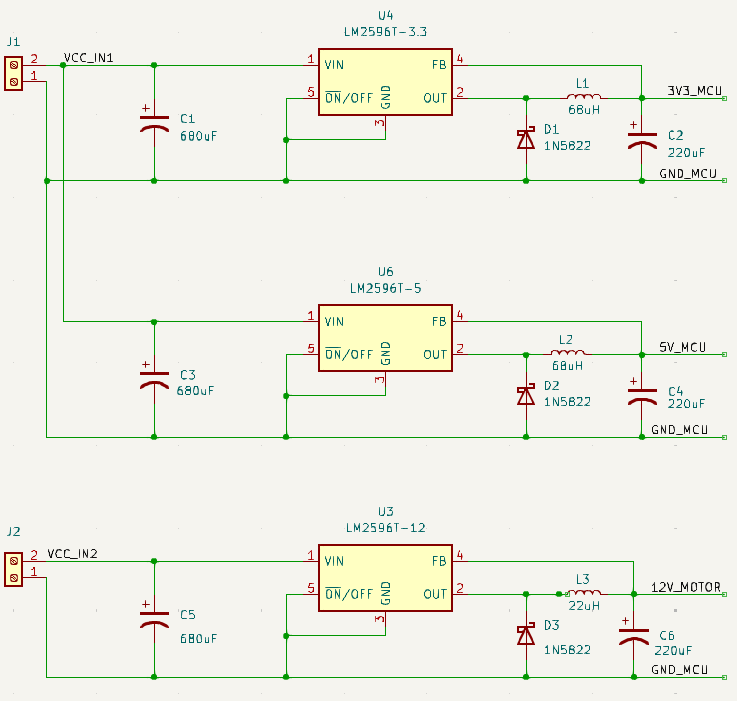
\includegraphics[width=1\textwidth]{pictures/chapter4/c4_p13_PowerSchematic.png}
                    \caption{Sơ đồ nguyên lý mạch nguồn}
                    \label{fig:4-9}
                \end{figure}
                \hspace*{0.6cm}Các linh kiện (điện trở, tụ điện, cuộn cảm) được chọn theo bảng từ tài liệu tham khảo \cite{lm2596}.
                \begin{itemize}
                    \item Với nguồn đầu ra 3.3V, nguồn đầu vào 7.4V và dòng tải không quá 3A, ta chọn: cuộn cảm $L = 22 \mu H$, tụ điện $C_{out} = 680 \mu F$. 
                    \item Với nguồn đầu ra 5V, nguồn đầu vào 7.4V và dòng tải không quá 3A, ta chọn: cuộn cảm $L = 22 \mu H$, tụ điện $C_{out} = 560 \mu F$.
                    \item Với nguồn đầu ra 12V, nguồn đầu vào 14.8V và dòng tải không quá 3A, ta chọn: cuộn cảm $L = 22 \mu H$, tụ điện $C_{out} = 470 \mu F$.
                    \item Chọn tụ điện đầu vào $C_{in} = 680 \mu F, V = 35 V$ cho cả 3 mạch vì $V_{C} = 35 V > 1.5 \times V_{max} = 1.5 \times 14.8 = 22.2 V$.
                \end{itemize}
        \section{Thiết kế mạch cho toàn bộ hệ thống}
            \subsection{Sơ đồ nguyên lý mạch toàn bộ hệ thống}
                \hspace*{0.6cm}Dựa vào các thiết kế mạch cảm biến, mạch nguồn và các linh kiện khác, ta thiết kế sơ đồ nguyên lý mạch toàn bộ hệ thống như sau:
                \begin{figure}[H]
                    \centering
                    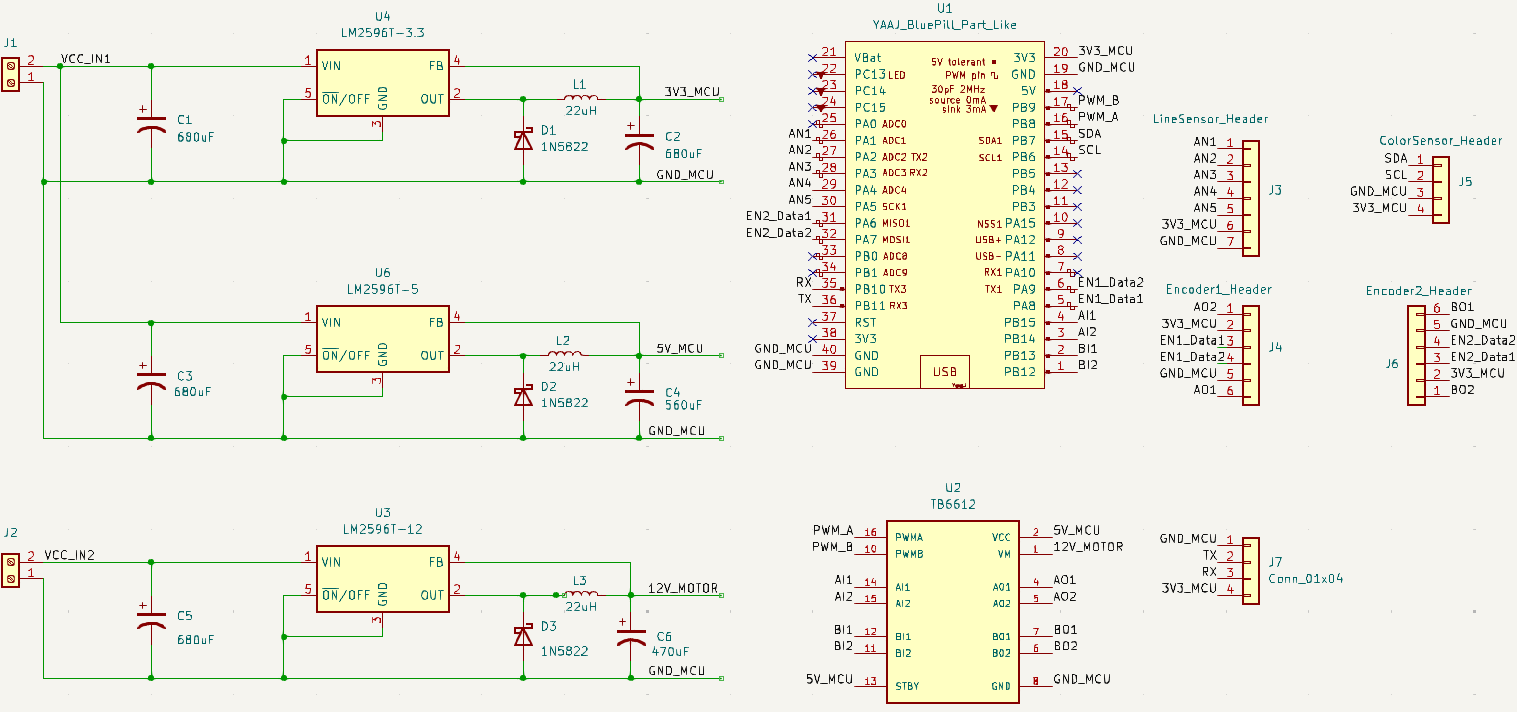
\includegraphics[width=0.95\textwidth]{pictures/chapter4/c4_p14_Schematic.png}
                    \caption{Sơ đồ nguyên lý mạch toàn bộ hệ thống}
                    \label{fig:4-17}
                \end{figure}
            \subsection{Thiết kế PCB mạch toàn bộ hệ thống}
                \hspace*{0.6cm}Dựa vào sơ đồ nguyên lý mạch toàn bộ hệ thống, ta tiến hành thiết kế PCB cho mạch toàn bộ hệ thống. Sơ đồ thiết kế PCB được trình bày như hình \ref{fig:4-18}.
                \begin{figure}[H]
                    \centering
                    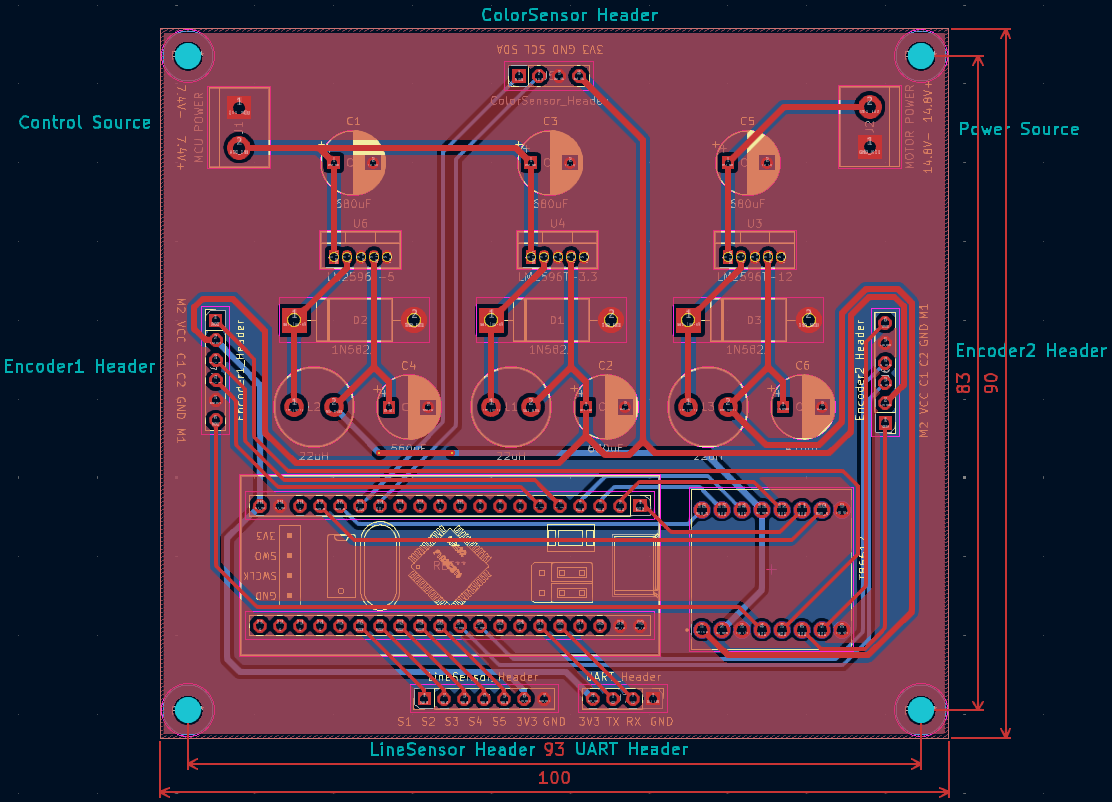
\includegraphics[width=0.8\textwidth]{pictures/chapter4/c4_p15_PCB.png}
                    \caption{Sơ đồ thiết kế PCB mạch toàn bộ hệ thống}
                    \label{fig:4-18}
                \end{figure}
            
                